%   ___             _         _          _
%  / __|___ _ _  __| |_  _ __(_)___ _ _ (_)
% | (__/ _ \ ' \/ _| | || (_-< / _ \ ' \| |
%  \___\___/_||_\__|_|\_,_/__/_\___/_||_|_|

% Slide 11 % % % % % % % %
\begin{frame}[plain]{\alert{Conclusioni}}
\label{frm:conclusioni:1}

  Lo stile Landmark, durante la navigazione Web, utilizza strategie simili a quelle adottate
  durante la navigazione in ambiente reale.
  \vspace{1em}

  Infatti, quando non e' sicuro della propria posizione, ritorna a un punto di riferimento
  precedente per provare un'altra strada \parencite{nori2010familiarity} e la stessa insicurezza si riflette anche durante la navigazione Web.
  \vspace{1em}

I risultati sono inoltre in linea con lo studio di \textcite{piccardi2016navigational} nel quale emerge un diverso pattern di movimenti oculari durante l'apprendimento di una mappa.
\end{frame}

\begin{frame}[plain]{\alert{Componenti Programma}}
  \begin{figure}
    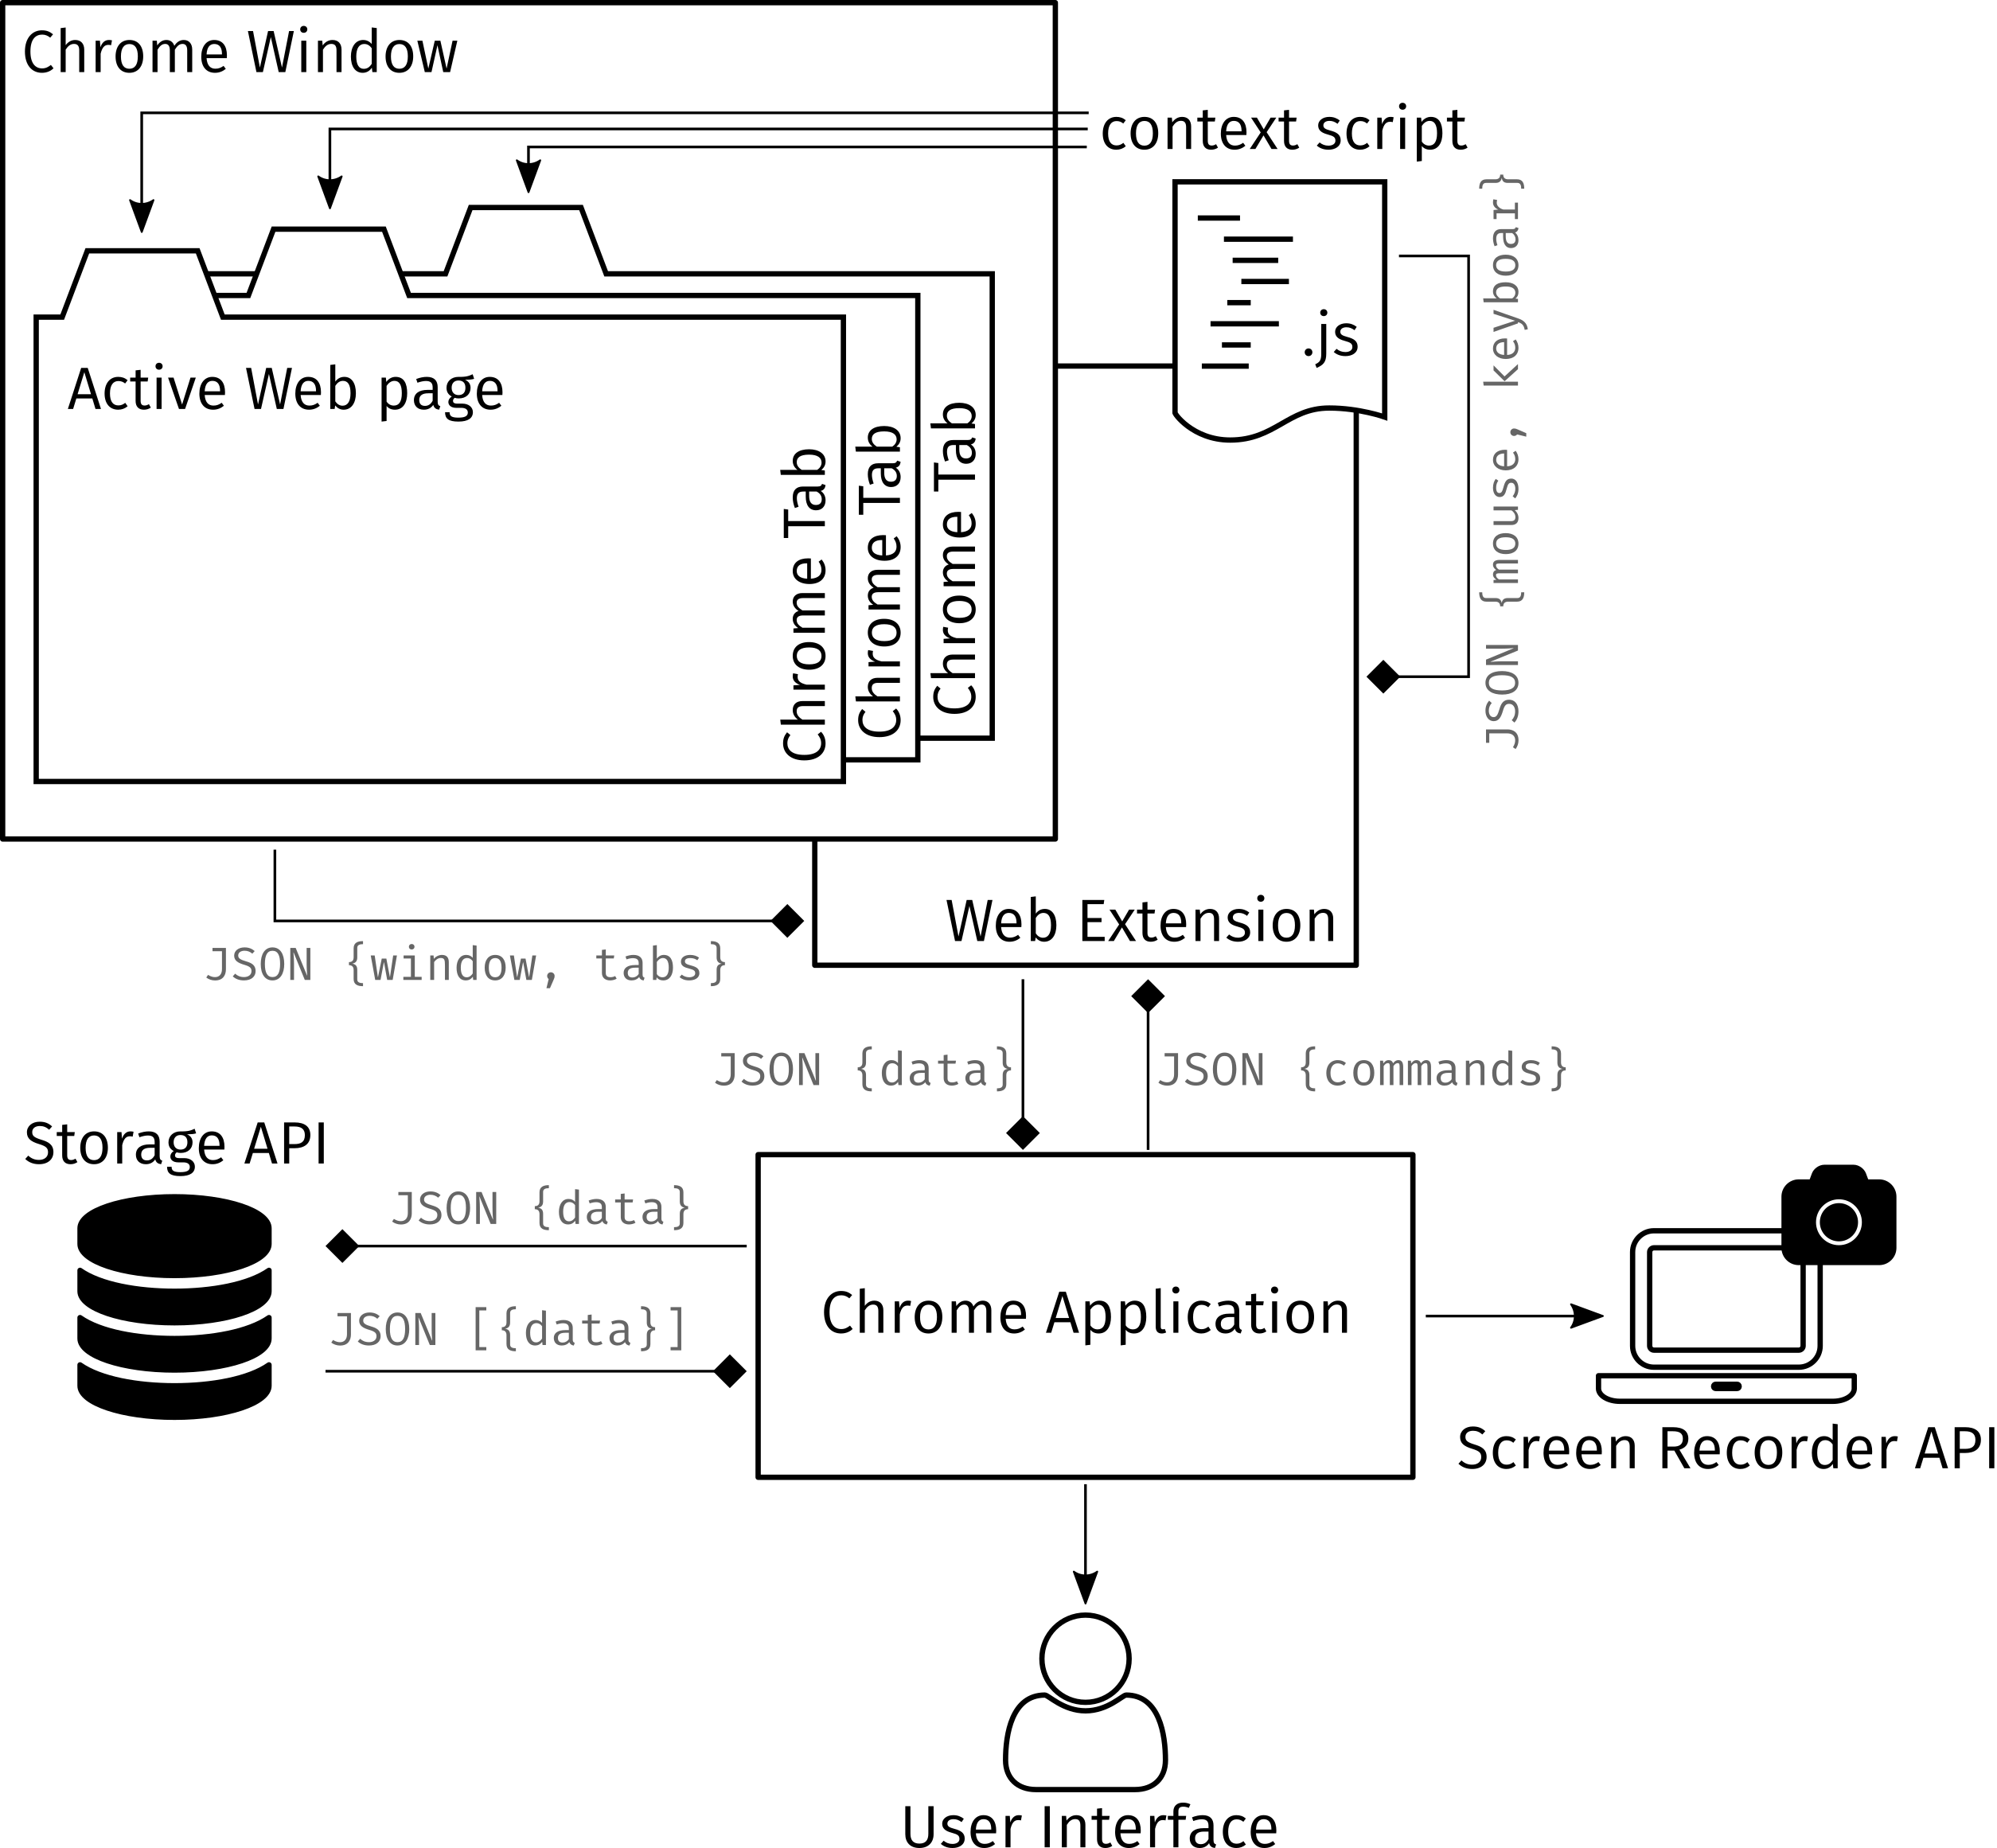
\includegraphics[height=0.8\textheight]{img/soft_scheme.png}
  \end{figure}
\end{frame}
